%% i don't think need to repeat what did in above section. 
%% that is important for a thesis chapter, but for a peer-reviewed paper, suggest we try to keep it as sucint (tight) as possible
%% a main comment throughout -- usually we use past tense when describing methods and results in most modeling papers. So would consider changing that here.
% nb: I have not changed verb tense in my edits
To examine the influence of turnover on epidemics, we first
compare equilibrium prevalence and incidence using models with and without:
population growth,
heterogeneity in risk, and
risk group turnover.
We then examine the influence of different rates of turnover on
overall and group-specific equilibrium prevalence and incidence.
Finally, we examine the influence of turnover on the contribution of the 
highest risk group to the overall epidemic - as measured by the 
transmission population attributable fraction (TPAF).
%%  suggest framing these as objective questions using precise verbs (like examine, determine, test, etc.) 
%%  rather than 'to highlight, etc' as that suggests description and not an experiment.
%%  also, use one terminology consistently throughout - e.g. turnover - rather than several. 
%%  In the intro, you can introduce the various ways people have conceptualized this, 
%%  but in general, good to use consistent and single terminology throughout to help the reader
%%  i.e. use either 'turnover' or 'risk group dynamics', etc. but not both after introduction. 
%% i find turnover easier to conceptualize; less words; and also restricts the use of term 'dynamics' in
%% reference to the epidemic dynamics, and not something else

% ==================================================================================================
\subsection{Model \& Simulations}\label{ss:model-sim}
We start with a deterministic 1-sex SIR model of transmission %% not sure if need to say 'start with'? is this not the "full model", so instead suggest = "we developed a deterministic..."
in a population with heterogeneity in risk.
The model is not representative of a specific infection but includes balancing contacts %% cite 'balancing contacts" 
as per sexually transmitted infections.
The model includes three health states:
susceptible~$\mathcal{S}$, infectious~$\mathcal{I}$, and recovered~$\mathcal{R}$
(Figure~\ref{fig:health-states}),
and $G = 3$ levels of risk:
high~$H$, medium~$M$, and low~$L$.
Risk strata are defined by different number of contacts per unit time
so that individuals in risk group $i$ are assumed to
form contacts at a rate $C_{i}$.
The probability $\rho$ of contact formation between individuals in group $i$
with individuals in risk group $k$ is
be proportionate to the total number of available contacts within each group: 
%% that we restricted our analyses to proportionate mixing is an important limitation
%% to talk about in discussion (and reference work on assortative vs. proportionate mixing from Boily, Garnett, etc.)
%% and in limitations, remember to hypothesize (and cite if available) how this assumption could influence the findings
\begin{equation}
  \rho_{ik} = \frac 
    {C_k x_k}
    {\sum_{\mathrm{k}}C_{\mathrm{k}} x_{\mathrm{k}}}
    \label{eq:rho}
\end{equation}
\begin{figure}
  \centering
  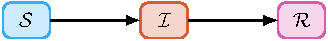
\includegraphics[width=0.4\linewidth]{health-states}
  \caption{Modelled health states.
  $\mathcal{S}$: susceptible;
  $\mathcal{I}$: infected;
  $\mathcal{R}$: recovered.}
  \label{fig:health-states}
\end{figure}
\par
The biological probability of transmission is defined as $\beta$ per contact. 
Individuals transition from the infectious $\mathcal{I}$ to susceptible $\mathcal{S}$ health-states  %% throughout - change 'infected' to 'infectious'.
via a force of infection per susceptible in risk group $i$
as shown:
\begin{equation}
  \lambda_{i} =
  C_{i} \sum_k \rho_{ik} \thinspace  \beta \thinspace \frac{\mathcal{I}_k}{x_k}
  \label{eq:foi}
\end{equation}

Individuals transition from the $\mathcal{I}$ are assumed to $\mathcal{R}$ health-state 
at a rate $\tau$ (per year), reflecting diagnosis and treatment.
Individuals in the $\mathcal{R}$ health-state are not infectious and are 
not susceptible. In this S-I-R system, individuals cannot become re-infected.
\par
As described in the previous section, individuals %% specify the exact section when mentioning 'previous section', etc.
enter the model at a rate $\nu$,
exit the model at a rate $\mu$,
and transition from risk group $i$ to group $j$ at a rate $\phi_{ij}$.
The turnover rates $\phi$ and distribution of model entrants by risk group $\bm{\hat{e}}$  %% what are 'model entrants'? - simplify terminology - its ok to use more words if the sentences are more clear that way
are resolved using the methods outlined in
Section \ref{sss:params-turnover}. %~\nameref{sss:params-turnover}.  %% why 'resolved' as a verb here? usually denotes there was a conflict? is there another verb we can use? 

%% i edited to try to simplify - and also to check that I understood what we are trying to say. If some of these are not correct, lets discuss so we can come up with the easiest language for co-authors to also understand
Our experiments were then carried out under the following pre-set conditions or assumptions.
First, we assumed that the proportion of individuals entering each risk group $\bm{\hat{e}}$ 
was equal to the proportion of individuals across risk groups in the $\bm{\hat{x}}$.
Second, we assumed that the average duration spent in each risk group $\bm{\delta}$ is known.
Third, the absolute number of individuals moving between two risk groups in either direction is balanced.
To meet all three conditions, there is only one possible value 
for each element in $\phi$ and $\bm{\hat{e}}$. In other words, by specifying these three conditions
we are able to identify and ensure that					%% simplify this sentence. remove 'to this end', etc. 
a unique set of $\phi$ and $\bm{\hat{e}}$ are determined.

The system of equations used to resolve $\phi$ and $\bm{\hat{e}}$  %% resolve or identify?
is given in \ref{aa:eqs-turnover}. %~\nameref{aa:eqs-turnover}.
\par
The above three assumptions help us define which parameters to use. The values of the parameters are generated from the data.
In this experiment, we use illustrative values as summarized in Table~\ref{tab:params-base}.
After resolving the system of equations,
$\bm{\hat{e}}$ is equal to $\bm{\hat{x}}$ (assumed),
and $\phi$ is:
\begin{equation}
\phi = \left[\begin{array}{ccc}
*      & 0.0833 & 0.0867 \\
0.0208 & *      & 0.0158 \\
0.0058 & 0.0042 & *      \\
\end{array}\right]
\end{equation}
The full system of model equations is given in \ref{aa:eqs-model}. %~\nameref{aa:eqs-model}.
\begin{table}
  \centering
  \caption{Base model parameters.
    All rates have units $\mathrm{year}^{-1}$ and durations are in $\mathrm{years}$.}
  \label{tab:params-base}
  \begin{tabular}{clc}
	\toprule
	    Symbol     & Description                                                             &                 Value                  \\
	\midrule
	 $\bm{\beta}$  & transmission probability per contact                                    &                 $0.03$                 \\
	    $\tau$     & rate of treatment initiation among infected                             &                 $0.1$                  \\
	    $N_0$      & initial population size                                                 &                 $1000$                 \\
	\midrule
	$\bm{\hat{x}}$ & proportion of system individuals: high, medium, low activity            & $[ 0.04 \enspace 0.20 \enspace 0.76 ]$ \\
	$\bm{\hat{e}}$ & proportion of entering individuals: high, medium, low activity          & $[ 0.04 \enspace 0.20 \enspace 0.76 ]$ \\
	$\bm{\delta}$  & average duration spent in: high, medium, and low activity groups        &    $[ 5 \enspace 15 \enspace 25 ]$     \\
	     $C$       & rate of contact formation among individuals: high, medium, low activity &     $[ 25 \enspace 5 \enspace 1 ]$     \\
	    $\nu$      & rate of population entry                                                &                 $0.05$                 \\
	    $\mu$      & rate of population exit                                                 &                 $0.03$                 \\
	\bottomrule
\end{tabular}
\end{table}
\par

We then simulate the base model, and the model variants, using these parameters.
We seed the epidemic with one infectious individual $\mathcal{I}$ in each risk group
at $t = 0$. The model starts with $N_0 = 1000$ individuals who are distributed across risk groups according to $\bm{\hat{x}}$.
There are no $\mathcal{R}$ at the start of the epidemic, and so all individuals except the 3 infectious individuals are susceptible $\mathcal{S}$.
We numerically solve the system of ordinary differential equations 
in Python%
\footnote{Code for all aspects of the project is available at:
  \href{https://github.com/c-uhs/turnover}{\texttt{https://github.com/c-uhs/turnover}}}
using Euler's method with a time step of $dt = 0.1$ years.

The model is assumed to be at equilibrium after $t = 500$ years,
which was verified qualitatively. % JK: another way of saying this?  %% SM: not sure what you want to say here?  Usually we say something like this:
%% All comparative analyses are then conducted at equilibrium, defined as a steady state with <X% difference in incidence.

% ==================================================================================================
\subsection{Model Variants}\label{ss:exp-variants}
To examine the influence of population growth, heterogeneity, and turnover,
we simplified the full model accordingly to include or remove each feature. 
These simplified model variants and their parameters are shown in Figure~\ref{fig:variant-tree},
and in Table~\ref{tab:params-variants}, respectively.
% Consider using "full model" instead of base model since each variant essentially removes from a full model - i.e. and does not add to a base model?
% Figure 3 starts with a base model at top and ends with a base model B. Suggest removing that first bit "Base Model"
% --------------------------------------------------------------------------------------------------
\paragraph{Experiment 1.1: Influence of risk heterogeneity}\label{p:exp-1-hetero}
V1 assumes no heterogeneity in risk and 
the V1 contact rate $C$ for all individuals equals the weighted 
average of the full model's risk-stratified $C_i$.						%suggest using V1, full model, etc. rather than 'previously' or 'new', etc. as that starts getting hard to follow
V1 does not have turnover because there is only one risk group.
All other conditions, including population growth rate, remain the same between
the full model and V1 (Table 2).

% No other parameters are changed as no other parameters
% were originally stratified by risk.
% --------------------------------------------------------------------------------------------------
\paragraph{Experiment 1.2: Influence of population growth}\label{p:exp-1-growth}
V2 assumes no population growth. The exit rate $\mu$ remains fixed and the same as the full model
but the entry rate $\nu$ is reduced to equal $\mu$.
This ensures that the average time spent in the modeled population $\mu^{-1}$ remains the same between the full model and V2. % it will not be clear what 'unchanged' means if we don't say what the comparator is. At first I thought it meant unchanged compared with V1 (which is correct, but I think we mean full model when we say unchanged?)
% --------------------------------------------------------------------------------------------------
\paragraph{Experiment 1.3: Influence of turnover}\label{p:exp-1-turnover}
V3 assumes there is no turnover, such that 
all turnover rates $\phi = 0$.
Following Eq.~(\ref{eq:duration-group}),
this means that in V3, the time spent within all risk groups is 
equal to the average duration of individuals in the model $\mu^{-1}$.
Since the distribution of risk behaviour in the entering population $\bm{\hat{e}}$		
%% we use different terminology/wording in section 3.1; it will be easier for the reader if we are consistent so lets revise this 
% E.g. The proportion of individuals who enter each risk group $\bm{\hat{e}}$ are equivalent to the distribution of the population by risk group $\bm{\hat{x}}$, no other modifications were needed. That is, the proportion of individuals in each risk group are the same across the full model, V2, and V3 (Table 2).
was assumed to be equal to that in the model $\bm{\hat{x}}$,
no other modifications are required.

\begin{figure}
  \centering
  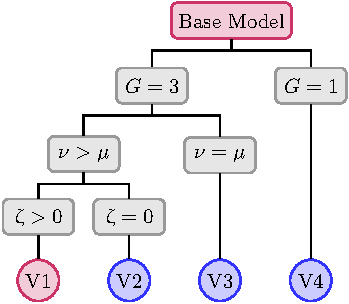
\includegraphics[width=0.7\linewidth]{variant-tree}
  \caption{Summary of the full model and three model variants
    with respect to heterogeneity in risk, population growth (pop. growth), and turnover.
    Relative population size of each risk group is the same in all variants.
    $G$:~number of risk groups,
    $\nu$:~rate of population entry,
    $\mu$:~rate of population exit,
    $\phi$:~rates of population turnover.}
  \label{fig:variant-tree}
\end{figure}
\begin{table}
  \centering
  \caption{Parameters for model variants.
    All rates have units $\mathrm{year}^{-1}$ and durations are in $\mathrm{years}$.
    Vectors correspond to parameters stratified by high, medium, and low risk groups.}
  \label{tab:params-variants}
  \begin{threeparttable}
\begin{tabularx}{0.95\linewidth}{c *{4}{Y}}
	\toprule
	  Parameter    & Full                     & V1                           & V2                       & V3                                         \\
	\midrule
	$\bm{\hat{x}}$ & $[ 0.05\es0.20\es0.75 ]$ & ---                          & $[ 0.05\es0.20\es0.75 ]$ & $[ 0.05\es0.20\es0.75 ]$                   \\
	$\bm{\hat{e}}$ & $[ 0.05\es0.20\es0.75 ]$ & ---                          & $[ 0.05\es0.20\es0.75 ]$ & $[ 0.05\es0.20\es0.75 ]$                   \\
	     $C$       & $[ 25\es5\es1 ]$         & $[ \textbf{3} ]$\tnote{a}    & $[ 25\es5\es1 ]$         & $[ 25\es5\es1 ]$                           \\
	   $\delta$    & $[ 5\es15\es25 ]$        & $[ \textbf{33.3} ]$\tnote{b} & $[ 5\es15\es25 ]$        & $[ \textbf{33.3\es33.3\es33.3} ]$\tnote{b} \\
	    $\nu$      & $0.05$                   & $0.05$                       & $\textbf{0.03}$\tnote{c} & $0.05$                                     \\
	    $\mu$      & $0.03$                   & $0.03$                       & $0.03$                   & $0.03$                                     \\
	\bottomrule
\end{tabularx}
\footnotesize
\begin{tablenotes}
  \item
  $\bm{\hat{x}}$: proportion of individuals in the model by risk group (high, medium, low);
  $\bm{\hat{e}}$: proportion of individuals entering the model by risk group;
  $C$: rate of contact formation by risk group (per year);
  $\delta$: average duration in each risk group (years);
  $\nu$: rate of population entry (per year);
  $\mu$: rate of exit (per year).
  \item[a] Weighted average of risk-stratified $C$
  \item[b] Without turnover, duration in all groups must be equal to the inverse of the exit rate, $\mu^{-1}$
  \item[c] Adjusting the entry rate, versus exit rate, does not affect average duration in the model
\end{tablenotes}
\end{threeparttable}
\end{table}

%% 'duration in the model' may not be clear to most people. change to 'duration or time spent in the modeled population'.
%% in the table title - the 'all rates have units year-1 and durations are in years' could go into the footnote I think or provide a written description of each parameter so its
%% easier to know if that parameter is a rate or a duration. i.e. just like Figure 3, without too many additional words - add a description of the parameter. Right now we have to go into the main text to figure it out :). 
% ==================================================================================================
\subsection{Influence of Turnover}\label{ss:exp-turnover}  %% frame the duration of infectiousness part as a sensitivity analysis
To further examine the influence of turnover on equilibrium prevalence and incidence, 
we varied the magnitude of turnover. We then conducted a sensitivity analysis   %% somewhere above, we say 'rates of turnover' - lets stick to one terminology throughout
to examine the influence of turnover at different treatment rates (durations of infectiousness).
% --------------------------------------------------------------------------------------------------
\paragraph{Experiment 2.1: Turnover Magnitude}
First, the magnitude of turnover is considered alone,
for fixed duration of infectiousness.
As in similar experiments \citep{Zhang2012,Henry2015},
the rates of turnover are scaled by a single parameter.
However, since the model used here has $G = 3$ risk groups,
it is not possible to simply multiply a set of base rates $\phi$ by a scalar factor;
this would result in changes to the equilibrium risk group sizes,
which is avoided throughout this work.
Rather, the rates of turnover are controlled by
the duration of individuals in the high risk group $\delta_H$ in the following way.
The distribution of model entrants $\bm{\hat{e}}$ is again assumed to equal
the distribution of individuals in the model $\bm{\hat{x}}$.
The absolute number of individuals moving between two groups in either direction
is also assumed to be balanced, as before.
% Then, the duration of individuals in the high risk group $\delta_H$
% is used as the controlling parameter.
The duration of individuals in the medium risk group $\delta_M$
is then defined as a value between $\delta_H$ and the maximum duration $\mu^{-1}$
which scales with $\delta_H$ following the equation:
$\delta_M = \delta_H + \kappa \left(\mu^{-1} - \delta_H\right)$, with $\kappa = 0.3$.
Finally, the duration of individuals in the low risk group $\delta_L$
similarly scales with $\delta_H$,
but the value is not required to resolve $\phi$;
it can be determined from $\phi$ afterwards
using Eq.~(\ref{eq:duration-group}).
In this way, each value of $\delta_H$ can be used to compute a set of turnover rates $\phi$
whose elements all scale inversely with the duration in the high risk group $\delta_H$.
The value of $\delta_H$ is then varied from 3~to~33 years,
and trends in the equilibrium incidence and prevalence are plotted
for each group, as well as overall.
%The duration in a risk group is also perhaps easier to grasp
%than individual transition rates.
%\footnote{Throughout this work,
%  we define duration $\delta_i$ as a ``single average pass through the group''
%  which does not consider reentrance after exiting to another group.}
% JK: I feel like these limits need justification,
% but its difficult to give without grounding in any specific infections
\par
% --------------------------------------------------------------------------------------------------
\paragraph{Experiment 2.2: Turnover and Treatment Rate}
Next, the above experiment is repeated for a range of treatment rates.
The treatment rate controls the duration of infectiousness $\delta_{\mathcal{I}}$
as in $\delta_{\mathcal{I}} = \tau^{-1}$.
Treatment rate $\tau$ is varied from 1~to~0.05,
implying a duration of infectiousness of 1~to~20 years.
The duration in the high risk group $\delta_H$ is varied from 3~to~33 years as before,
and trends equilibrium incidence and prevalence are again shown,
this time using 2D surface plots.
% ==================================================================================================
\subsection{Implications for Model Fitting}\label{ss:exp-turnover-fit}
Finally, since almost all context-specific applications of epidemic models entail
fitting uncertain model parameters to data-driven calibration targets,
some potential implications of omitting turnover from a fitted model are explored.
In particular, the influence of turnover on two model outputs are estimated,
before and after model fitting:
the inferred level of risk heterogeneity in the population;
and the transmission population attributable fraction (TPAF)~\citep{Mishra2016}
of the high risk group.
TPAF estimates the proportion of cumulative new infections which are attributable to
prevention gaps among a specific population.%
\footnote{To estimate TPAF of the high risk group,
  transmission ``from'' the high risk group is turned off, not ``to''.}
% --------------------------------------------------------------------------------------------------
\paragraph{Experiment 3.1: Inferred Risk Heterogeneity}
First, the Base model (turnover) and model variant V3 (no~turnover) are both calibrated to
25\% prevalence in the high risk group, and
5\% prevalence in the low risk group at equilibrium.
The fitted parameters are
the contact rates of the high and low risk groups: $C_H$~and~$C_L$.%
\footnote{The fitted parameters are estimated by minimizing
  the negative log-likelihood of each predicted prevalence versus the target
  (assuming a sample size of 1000)
  using the Sequential Least SQuares Programming (SLSQP) method~\citep{Kraft1988}
  from the \texttt{scipy.optimize.minimize} Python package.}
The ratio of fitted contact rates $C_H~/~C_L$
represents the degree of risk heterogeneity in the population
which must be present in order to observe the given prevalence ratio.
Comparing the fitted contact rates with and without turnover,
the influence of turnover on inferred risk heterogeneity is shown.
% --------------------------------------------------------------------------------------------------
\paragraph{Experiment 3.2: TPAF of the High Risk Group}
The level of risk heterogeneity has presumed implications
for prioritization of risk groups for interventions.
The TPAF of a risk group provides an estimate of
the importance of prioritizing the group.
Thus, differences in inferred risk heterogeneity due to turnover from Experiment 3.1
are hypothesized to result in differences in the estimated TPAF of the high risk group.
To test this hypothesis, the TPAF of the high risk group
is calculated and compared across the model variants with and without turnover,
before and after fitting to group-specific prevalence, as described above.